\documentclass[11pt]{article}
\usepackage{latexsym}
\usepackage{amsmath}
\usepackage{amssymb}
\usepackage{amsthm}
\usepackage{epsfig}
\usepackage{graphicx}

\usepackage{amsmath}
\usepackage{amssymb}
\newcommand{\hw}[3]{
	\noindent
	\begin{center}
		\framebox{
			\vbox{
				\hbox to 5.78in { {\bf CSCE 653: Computational Methods for Data Science} \hfill  }
				\vspace{2mm}
				\hbox to 5.78in { {\Large \hfill Homework #1\hfill} }
				\vspace{2mm}
				\hbox to 5.78in { {\it Due date: #2 \hfil Name: #3} }
			}
		}
	\end{center}
	\vspace*{4mm}
}

%Problems, Answers and Solutions
\newcounter{prob}
\setcounter{prob}{-1}
\newcommand{\problem}{\stepcounter{prob}{\noindent\textbf{Problem \theprob.}}\ }
\newcommand{\answer}{\medskip{\color{red} \textbf{Answer to Problem \theprob.}}\ }
\newcommand{\solution}{\medskip{\color{blue} \textbf{Solution to Problem \theprob.}}\ }

%New commands
\def\ds{\displaystyle}
\def\ra{\rightarrow}
%\def\bf{\textbf}
\usepackage{enumerate}
\newcommand{\babc}{\begin{enumerate}[a)]} %Use with \item for abc lists
\newcommand{\eabc}{\end{enumerate}}


% For hyperlinking everything
\usepackage{hyperref}
\hypersetup{
	colorlinks=true, %set true if you want colored links
	linktoc=all,     %set to all if you want both sections and subsections linked
	linkcolor=blue,  %choose some color if you want links to stand out
}

\usepackage{tabularx}
\usepackage{booktabs}
\usepackage[latin1]{inputenc}
\usepackage{amsmath}
\usepackage{mathrsfs}  
\usepackage{amsfonts}
\usepackage{amssymb}
\usepackage{graphicx}
\usepackage{subfig}
\usepackage{caption}
\usepackage{algorithm}
%\usepackage{algcompatible}
%\usepackage{algorithmicx}
\usepackage{algpseudocode}
%\usepackage{enumitem}
\usepackage{color}
\usepackage{titlesec}
\titleformat{\section}{\fontfamily{lmss}\fontsize{14}{15}\bfseries}{\thesection}{1em}{}
\titleformat{\subsection}{\fontfamily{lmss}\fontsize{12}{15}\bfseries}{\thesubsection}{1em}{}

\usepackage{amsthm}

\newtheoremstyle{noit}
{10pt}% <Space above>
{10pt}% <Space below>
{}% <Body font>
{}% <Indent amount>
{\bfseries}% <Theorem head font>
{.}% <Punctuation after theorem head>
{.5em}% <Space after theorem headi>
{}% <Theorem head spec (can be left empty, meaning `normal')>

\newtheoremstyle{example}
{10pt}% <Space above>
{10pt}% <Space below>
{}% <Body font>
{20pt}% <Indent amount>
{\bfseries}% <Theorem head font>
{.}% <Punctuation after theorem head>
{.5em}% <Space after theorem headi>
{}% <Theorem head spec (can be left empty, meaning `normal')>


\newtheoremstyle{indented}{20pt}{20pt}{\addtolength{\leftskip}{2.5em}}{}{\bfseries}{.}{.5em}{}

%\theoremstyle{indented}
\newtheorem{claim}{Claim}
\newtheorem{theorem}{Theorem}
\numberwithin{theorem}{section}
\newtheorem{lemma}[theorem]{Lemma}
\newtheorem{corollary}[theorem]{Corollary}
\newtheorem{observation}{Observation}
%\numberwithin{observation}{section}
%\numberwithin{definition}{section}
\newtheorem{conjecture}{Conjecture}
\newtheorem{Qu}{Question}
\newcommand{\QU}{\begin{Qu}\normalfont}
	
	\newtheorem{definition}{Definition}
	
	\theoremstyle{noit}
	\newtheorem{fact}{Fact}
	
	%\theoremstyle{indented}
	
	
	\theoremstyle{indented}
	\newtheorem{example}{Example}
	
	\theoremstyle{indented}
	%\newtheorem{problem}{Problem}
	
	
	\newcommand{\vs}[1]{\vspace{#1}}
	
	\newcommand{\lecture}[1]{
		\noindent
		\begin{center}
			\framebox{
				\vbox{
					\hbox to 5.78in { {\bf CSCE 653: Computational Methods for Data Science} \hfill  }
					\vspace{2mm}
					\hbox to 5.78in { {\Large \hfill Lecture #1\hfill} }
					\vspace{2mm}
					\hbox to 5.78in { {Texas A\&M University \it  \hfill Lecturer: Nate Veldt} }
				}
			}
		\end{center}
		\vspace*{4mm}
	}
	
	
	\newcommand{\under}[1]{\underline{\hspace{#1}}}
	\setlength{\parindent}{0em}
	
	\newcommand\norm[1]{\left\lVert#1\right\rVert}
	\newcommand\normx[1]{\left\Vert#1\right\Vert}
	
	% Graph terms
	\newcommand{\vol}{\textbf{vol}}
	\newcommand{\cut}{\textbf{cut}}
	%\newcommand{\span}{\textbf{span}}
	
	% Matrices
	\newcommand{\mL}{\textbf{L}}
	\newcommand{\mR}{\textbf{R}}
	\newcommand{\mA}{\textbf{A}}
	\newcommand{\mB}{\textbf{B}}
	\newcommand{\mC}{\textbf{C}}
	\newcommand{\mM}{\textbf{M}}
	\newcommand{\mP}{\textbf{P}}
	\newcommand{\mZ}{\textbf{Z}}
	\newcommand{\mY}{\textbf{Y}}
	\newcommand{\mX}{\textbf{X}}
	\newcommand{\mI}{\textbf{I}}
	\newcommand{\mH}{\textbf{H}}
	\newcommand{\mW}{\textbf{W}}
	\newcommand{\mV}{\textbf{V}}
	\newcommand{\mU}{\textbf{U}}
	\newcommand{\mQ}{\textbf{Q}}
	% vectors
	
	\DeclareMathOperator*{\argmax}{argmax}
	\DeclareMathOperator*{\argmin}{argmin}
	
	\newcommand{\blue}[1]{{\color{blue} #1 }}
	\newcommand{\va}{\textbf{a}}
	\newcommand{\vb}{\textbf{b}}
	\newcommand{\vc}{\textbf{c}}
	\newcommand{\vd}{\textbf{d}}
	\newcommand{\ve}{\textbf{e}}
	\newcommand{\vh}{\textbf{h}}
	\newcommand{\vw}{\textbf{w}}
	\newcommand{\vl}{\textbf{l}}
	\newcommand{\vp}{\textbf{p}}
	\newcommand{\vq}{\textbf{q}}
	\newcommand{\vr}{\textbf{r}}
	\newcommand{\vu}{\textbf{u}}
	\newcommand{\vv}{\textbf{v}}
	\newcommand{\vx}{\textbf{x}}
	\newcommand{\vy}{\textbf{y}}
	\newcommand{\vz}{\textbf{z}}
	\newcommand{\zvec}{\textbf{0}}
	% Other
	\newcommand{\calN}{\mathcal{N}}
	\newcommand{\tr}{\text{tr}}
	\usepackage{mathtools}
	\DeclarePairedDelimiter\ceil{\lceil}{\rceil}
	\DeclarePairedDelimiter\floor{\lfloor}{\rfloor}
	\DeclareMathOperator{\EX}{\mathbb{E}}% expected value

	
	\newcommand{\note}[1]{{\color{blue} [ #1 ]}}
	\newcommand{\hide}[1]{\underline{\phantom{#1 #1}}}
	
	\newcommand{\R}{\mathbb{R}}
	\newcommand{\Rn}{\mathbb{R}^n}
	\newcommand{\Rnn}{\mathbb{R}^{n \times n}}
	\usepackage{setspace}

\usepackage[T1]{fontenc}
\usepackage{beramono}
\usepackage{listings}
\usepackage[usenames,dvipsnames]{xcolor}

%%
%% Julia definition (c) 2014 Jubobs
%%
\lstdefinelanguage{Julia}%
  {morekeywords={abstract,break,case,catch,const,continue,do,else,elseif,%
      end,export,false,for,function,immutable,import,importall,if,in,%
      macro,module,otherwise,quote,return,switch,true,try,type,typealias,%
      using,while},%
   sensitive=true,%
   alsoother={$},%
   morecomment=[l]\#,%
   morecomment=[n]{\#=}{=\#},%
   morestring=[s]{"}{"},%
   morestring=[m]{'}{'},%
}[keywords,comments,strings]%

\lstset{%
    language         = Julia,
    basicstyle       = \ttfamily,
    keywordstyle     = \bfseries\color{blue},
    stringstyle      = \color{magenta},
    commentstyle     = \color{ForestGreen},
    showstringspaces = false,
}


\newcommand{\handout}[5]{
  \noindent
  \begin{center}
  \framebox{
    \vbox{
      \hbox to 5.78in { {\bf Numerical Linear Algebra } \hfill #2 }
      \vspace{4mm}
      \hbox to 5.78in { {\Large \hfill #5  \hfill} }
      \vspace{2mm}
      \hbox to 5.78in { {\em #3 \hfill #4} }
    }
  }
  \end{center}
  \vspace*{4mm}
}

\newcommand{\topic}[4]{\handout{#1}{#2}{#3}{Scribe: #4}{Topic: #1}}
\newtheorem{assumption}[theorem]{Assumption}

% 1-inch margins, from fullpage.sty by H.Partl, Version 2, Dec. 15, 1988.
\topmargin 0pt
\advance \topmargin by -\headheight
\advance \topmargin by -\headsep
\textheight 8.9in
\oddsidemargin 0pt
\evensidemargin \oddsidemargin
\marginparwidth 0.5in
\textwidth 6.5in

\parindent 0in
\parskip 1.5ex
%\renewcommand{\baselinestretch}{1.25}

\begin{document}

\topic{Fundamentals}{\today}{FAUST}{David Zhang}

\section{Vandermonde Matrix}

\definition{A \textbf{Vandermonde matrix} is a matrix with the terms of a geometric progression in each row, i.e.:}
\begin{align*}
\begin{bmatrix}
1 & x_1 & x_1^2 & \cdots & x_1^{n-1} \\
1 & x_2 & x_2^2 & \cdots & x_2^{n-1} \\
\vdots & \vdots & \vdots & \ddots & \vdots \\
1 & x_m & x_m^2 & \cdots & x_m^{n-1}
\end{bmatrix}
\end{align*}

If c is a column vector of coefficients, then the product of the Vandermonde matrix and c is a column vector of the values of the polynomial at the points $x_1, x_2, \ldots, x_m$.

Thus the product $(Ac)_i = p(x_i)$ where $p(x)$ is the polynomial defined by the coefficients in c.

\section {Orthogonal Vectors and Matrices}


\begin{definition}
  A hermitian conjugate or adjoint of an $m \times n$ matrix $A$ is the $n \times m$ matrix $A^*$ obtained by taking the complex conjugate of each entry and then taking the transpose.

  \begin{align*}
    A^* = \overline{A}^T
  \end{align*}
    Where $$A^* = \begin{bmatrix}
    \overline{a_{11}} & \overline{a_{21}} & \cdots & \overline{a_{m1}} \\
    \overline{a_{12}} & \overline{a_{22}} & \cdots & \overline{a_{m2}} \\
    \vdots & \vdots & \ddots & \vdots \\
    \overline{a_{1n}} & \overline{a_{2n}} & \cdots & \overline{a_{mn}}
  \end{bmatrix}$$
\end{definition}

If $A = A^*$, then $A$ is said to be hermitian.

\begin{definition}
  An inner product is bilinear, meaning
  \begin{align*}
    (x_1 + x_2)y = x_1y + x_2y \\
    x(y_1 + y_2) = xy_1 + xy_2 \\
    (\alpha x)(\beta y) = \alpha \beta xy
  \end{align*}
\end{definition}

\begin{theorem}
  The vectors in an orthogonal set S are linearly independent.

  \begin{proof}
  Suppose $\alpha_1 v_1 + \cdots + \alpha_k v_k = 0$ for an orthogonal set $\{v_1, \dots, v_k\}$. By bilinearity of the inner product,
  \[
  0 
  = \langle \alpha_1 v_1 + \cdots + \alpha_k v_k, v_i \rangle 
  = \alpha_1 \langle v_1, v_i \rangle + \dots + \alpha_k \langle v_k, v_i \rangle.
  \]
  Since $\langle v_j, v_i \rangle = 0$ for $j \neq i$, we get
  \[
  \alpha_i \langle v_i, v_i \rangle = 0 \quad \implies \quad \alpha_i = 0.
  \]
  Hence, all $\alpha_i$ must be zero and the vectors are linearly independent.
  \end{proof}
\end{theorem}

Key idea:

Inner products and Orthogonality can decompose arbitrary vectors into orthogonal components.

\begin{theorem}
  If $q_1, \dots, q_n$ are orthogonal, then
  where $v$ is an arbitrary vector, and $q^Tv$ is a scalar.

  The vector $r = v - (q_1v)q_1 - \cdots - (q_nv)q_n$ is orthogonal to $q_1, \dots, q_n$.

  Multiplying $q_i$ by $r$ gives
  \begin{align*}
    q_i r &= q_i v - (q_i q_1)vq_1 - \cdots - (q_i q_n)vq_n \\
    &= q_i v - q_i v q_i q_i \\
    &= 0
  \end{align*}
\end{theorem}

\section{Norms}

Certain norms are more useful than other norms. These are the induced matrix norms,
defined in terms of the behavior of a matrix as an operator between its normed domain and 
range spaces.

The induced norm $\norm{A}_(m, n)$ of a matrix $A$ is defined as the smallest
number $C$ such that
\begin{align*}
  \norm{A}_(m, n) \leq C \norm{x}_n
\end{align*}

Otherwise, this is the 
\begin{align*}
  \norm{A}_(m, n) = \sup_{x \neq 0} \frac{\norm{Ax}_m}{\norm{x}_n} = \sup_{\norm{x}_n = 1} \norm{Ax}_m
\end{align*}

\definition{Cauchy-Schwarz and Holder's Inequality}

\begin{align*}
  \langle x, y \rangle \leq \norm{x}_2 \norm{y}_2
\end{align*}

\begin{align*}
  \norm{xy}_1 \leq \norm{x}_p \norm{y}_q
\end{align*}

where $p$ and $q$ are conjugate exponents (i.e. $\frac{1}{p} + \frac{1}{q} = 1$). Other than $p=q$, this is possible for any $p>1$ (e.g. $p=3, q=\tfrac{3}{2}$).

\section{Singular Value Decomposition}

If you don't know what to do, take the SVD

\begin{align*}
  A = U \Sigma V^*
\end{align*}

The left singular values U represent the length of the semiaxises of an ellipsoid, 
where the right singular values V the preimages of the principal semiaxes.

\begin{figure}[ht]
  \centering
  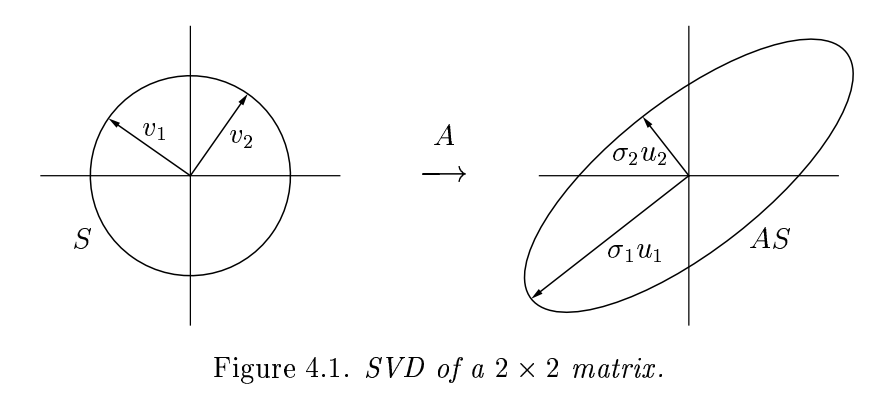
\includegraphics[width=0.5\textwidth]{SVD_Circle.png}
  \caption{SVD Circle Illustration}
  \label{fig:svd-circle}
\end{figure}

\section{More on SVD}

\definition{Nondefective Matrix}

A matrix is nondefective if it has a full set of eigenvectors.

\begin{theorem}
  Matrix A can be made as the sum of r rank-one matrices
  \begin{align*}
    A = \sum_{i=1}^r \sigma_i u_i v_i^*
  \end{align*}
\end{theorem}
The partial sums of the SVD are the best rank-r approximation to A. (the best energy)

%\bibliography{mybib}
\bibliographystyle{alpha}

\begin{thebibliography}{77}

\bibitem{fks}
Lloyd N. Trefethen, David Bau III,
\emph{Numerical Linear Algebra},
Northwestern University.


\end{thebibliography}

\end{document}